%!TEX root = forallxadl.tex
\part{Interpretations}
\label{ch.semantics}
\addtocontents{toc}{\protect\mbox{}\protect\hrulefill\par}


\chapter{Extensionality}\label{s:Interpretations}

Recall that \TFL\ is a truth-functional language. Its connectives are all truth-functional, and \emph{all} that we can do with \TFL\ is key sentences to particular truth values. We can do this \emph{directly}. For example, we might stipulate that the \TFL\ sentence `$P$' is to be true. Alternatively, we can do this \emph{indirectly}, offering a symbolisation key, e.g.:
	\begin{ekey}
		\item[P] Big Ben is in London
	\end{ekey}
But recall from §\ref{s:TruthFunctionality} that this should be taken to mean:
	\begin{itemize}
		\item The \TFL\ sentence `$P$' is to take the same truth value as the English sentence `Big Ben is in London' (whatever that truth value may be)
	\end{itemize}
The point that I emphasised is that \TFL\ cannot handle differences in meaning that go beyond mere differences in truth value.


\section{Symbolising versus translating}
\FOL\ has some similar limitations. It gets beyond mere truth values, since it enables us to split up sentences into terms, predicates and quantifier expressions. This enables us to consider what is \emph{true of} some particular object, or of some or all objects. But we can do no more than that. 

When we provide a symbolisation key for some \FOL\ predicates, such as:
	\begin{ekey}
		\item[C] \gap{1} lectures on logic in Adelaide in Semester 2, 2018
	\end{ekey} 
we do not carry the \emph{meaning} of the English predicate across into our \FOL\ predicate. We are simply stipulating something like the following:
	\begin{itemize}
		\item `$C$' and `\gap{1} lectures on logic in Adelaide in Semester 2, 2018' are to be \emph{true of} exactly the same things. 
	\end{itemize}
So, in particular:
	\begin{itemize}
		\item `$C$' is to be true of all and only those things which lecture on logic in Adelaide in Semester 2, 2018 (whatever those things might be).
	\end{itemize}
This is an indirect stipulation. Alternatively we can stipulate predicate extensions directly. We can stipulate that `$C$' is to be true of Antony Eagle and Jon Opie, and only them. As it happens, this direct stipulation would have the same effect as the indirect stipulation. But note that the English predicates `\blank\ is Antony Eagle or Jon Opie' and `\blank\ lectures on logic in Adelaide in Semester 2, 2018' have very different meanings!

The point is that \FOL\ does not give us any resources for dealing with nuances of meaning. When we interpret \FOL, all we are considering is what the predicates are actually true of. For this reason, I say only that \FOL\ sentences \emph{symbolise} English sentences. It is doubtful that we are \emph{translating} English into \FOL, for translations should preserve meanings.

This is normally summed up by saying that \FOL\ is an \define{extensional language}. The extension of an English expression is just the things to which it actually applies. So the extension of a name is the thing actually named; and the extension of a predicate is just those things it actually covers. An extensional language is one where expressions with the same extension are \emph{synonyms}. English is not an extensional language. In English, there is a distinction between the extension of a term – or what it \emph{denotes} – and what it \emph{means}. While the name `Scott Morrison' and the definite noun phrase `the Prime Minister' have the same extension, they are not synonyms. For one can replace an expression in a sentence by one of its synonyms, and the resulting sentence will mean the same thing as the original - and will have the same truth value. But while `Malcom Turnbull has always been Scott Morrison' is true, `Scott Morrison has always been the Prime Minister' is not true.\footnote{The previous iteration of this book used the name `Malcolm Turnbull' in this example.} Despite having the same extension, these expressions differ in meaning. In \FOL, by contrast, the substitition of one name for another with the same extension will always yield a sentence with the same truth-value; likewise with the substitution of one predicate for another with the same extension.\footnote{What this shows, in passing, is that \FOL\ lacks the resources to express things like `\gap{} has always been \gap{}' or `\gap{} is necessarily \gap{}', which would allow us to separate non-synonymous expressions with the same present extension. 

Another construction with apparently similar effects is when a true identity, such as `Lewis Carroll is Charles Lutwidge Dodgson', is embedded in a belief report such as `AE believes that Lewis Carroll is Charles Lutwidge Dodgson'. The belief report appears to be false, if AE doesn't know that `Lewis Carroll' is a pen name for the Oxford mathematician. But still, this seems hard to deny: `AE believes that Lewis Carroll is Lewis Carroll'. Many have used this to argue that the meaning of a name in English is not just its extension. But this is actually a rather controversial case, unlike the example in the main text: many philosophers think that the meaning of a name in English just is its extension. But let us be clear: no one generalises this to predicates. Everyone agrees that the meaning of an English predicate is not just its extension.}





\section{A word on extensions}
We can stipulate directly which things in our domain our predicates are to be true of. So it is worth noting that our stipulations can be as arbitrary as we like. For example, we could stipulate that `$H$' should be true of, and only of, the following objects:
	\begin{center}
		David Cameron\\
		the number $\pi$\\
		every top-F key on every piano ever made
	\end{center}
Now, the objects that we have listed have nothing particularly in common. But this doesn't matter. Logic doesn't care about what strikes us mere humans as `natural' or `similar'. Armed with this interpretation of `$H$', suppose I now add to my symbolisation key:
	\begin{ekey}
		\item[d] David Cameron
		\item[n] Julia Gillard
		\item[p] the number $\pi$
	\end{ekey}
Then `$Hd$' and `$Hp$' will both be true, on this interpretation, but `$Hn$' will be false, since Julia Gillard was not among the stipulated objects. 

This process of explicit stipulation is just giving the extension of a predicate by a list of items falling under it. The much more common way of identifying the extension of a predicate is to derive it from a classification rule that sorts everything into those items that fall under it and those that do not. Such a classification rule is often what people think of as the meaning of a predicate. 


\section{Many-place predicates}
All of this is quite easy to understand when it comes to one-place predicates. But it gets much messier when we consider two-place predicates. Consider a symbolisation key like:
	\begin{ekey}
		\item[L] \gap{1} loves \gap{2}
	\end{ekey}
Given what I said above, this symbolisation key should be read as saying:
	\begin{itemize}
		\item `$L$' and `\gap{1} loves \gap{2}' are to be true of exactly the same things in the domain
	\end{itemize}
So, in particular:
	\begin{itemize}
		\item `$L$' is to be true of a and b (in that order) iff a loves b. 
	\end{itemize}
It is important that we insist upon the order here, since love – famously – is not always reciprocated. (Note that `a' and `b' here are symbols of English, and that they are being \emph{used} to talk about particular things in the domain.)

That is an indirect stipulation. What about a direct stipulation? This is slightly harder. If we \emph{simply} list objects that fall under `$L$', we will not know whether they are the lover or the beloved (or both). We have to find a way to include the order in our explicit stipulation. 

To do this, we can specify that two-place predicates are true of \define{ordered pairs} of objects, which differ from two-membered collections in that the order of a pair is important. Thus we might stipulate that `$B$' is to be true of, and only of, the following pairs of objects:
	\begin{center}
		\ntuple{Lenin, Marx}\\
		\ntuple{Heidegger, Sartre}\\
		\ntuple{Sartre, Heidegger}
	\end{center}
Here the angle-brackets keep us informed concerning order – $\ntuple{a,b}$ is a different pair from $\ntuple{b,a}$ even though they correspond to the same collection of two things, a and b. Suppose I now add the following stipulations:
	\begin{ekey}
		\item[l] Lenin
		\item[m] Marx
		\item[h] Heidegger
		\item[s] Sartre
	\end{ekey}
Then `$Blm$' will be true, since \ntuple{Lenin, Marx} was in my explicit list. But `$Bml$' will be false, since \ntuple{Marx, Lenin} was not in my list. However, both `$Bhs$' and `$Bsh$' will be true, since both \ntuple{Heidegger, Sartre} and \ntuple{Sartre, Heidegger} are in my explicit list 

To make these ideas more precise, we would need to develop some \emph{set theory}, the mathematical theory of collections. This would give you some tools for modelling extensions and ordered pairs (and ordered triples, etc.). Indeed, set theoretic tools lie at the heart of contemporary linguistic approaches to meaning in natural languages. However, we have neither the time nor the need to cover set theory in this book. I shall leave these notions at an imprecise level; the general idea will be clear enough, I hope. 


\section{Semantics for identity}
Identity is a special predicate of \FOL. We write it a bit differently than other two-place predicates: `$x=y$' instead of `$Ixy$' (for example). More important, though, its meaning is fixed as to be genuine \emph{identity}, once and for all. Given a domain, the extension of `$=$' comprises just those pairs consisting of any member of the domain and itself. If the domain is numbers, for example, the extension of `$=$' on this domain will be $$\ntuple{1,1}, \ntuple{2,2}, \ntuple{3,3},….$$ 

If two names \meta{a} and \meta{b} are assigned to the same object in a given symbolisation key, and thus have the same extension, $\meta{a}=\meta{b}$ will also be true  on that symbolisation key. And since the two names have the same extension, and \FOL\ is extensional, substituting one name for another will not change the truth value of any \FOL\ sentence. So, in particular, if `$a$' and `$b$' name the same object, then all of the following will be true:\label{model.nonidentity}
	\begin{align*}
	 	Aa &\eiff Ab \\
	 	Ba &\eiff Bb\\
		Raa &\eiff Rbb\\
		Raa & \eiff Rab\\
		Rca &\eiff Rcb\\
		\forall x Rxa &\eiff \forall x Rxb
	\end{align*}
This fact is sometimes called the \define{indiscernibility of identicals} – if two names denote the same thing, then no claim will be true when formulated using one of those names but false when formulated using the other in its place. That is because, at the level of extensions, there really is just one thing that those claims are about, and how could that one thing be discernible from itself?

The converse claim – the \define{identity of indiscernibles} – is much more controversial. It is not defensible in \FOL. Suppose two objects differ in some property $\mathfrak{F}$, but our symbolisation key includes no predicate which denotes $\mathfrak{F}$. Then we might not have any sentence true of the one object and false of the other, even though they are \emph{distinct} objects which have different properties. We can't tell them apart, not because they are really just one, but because we don't have the right words to talk about how they are different. \FOL\ thus allows that exactly the same predicates might be true of two distinct objects, and thus they are distinct but indiscernible when restricted to the resources of our symbolisation.




\section{Interpretations} \label{ss.int}
I defined a \emph{valuation} in \TFL\ as any assignment of truth and falsity to atomic sentences. In \FOL, I am going to define an \define{interpretation} as consisting of three things:
	\begin{itemize}	
		\item the specification of a domain;
		\item for each name that we care to consider, an assignment of exactly one object within the domain as its extension;
		\item for each non-logical $n$-place predicate $\meta{A}$ (i.e., any predicate other than `$=$') that we care to consider, a specification of its extension: what things (or pairs of things, or triples of thing, etc.) the predicate is to be true of – where all those things must be in the domain.
	\end{itemize}
A $0$-place predicate (what we called `atomic sentences' in \TFL) has a truth value, either T or F, as its extension – thus the valuations of \TFL\ are intepretations of a very restricted part of \FOL\ – those interpretations which only care to consider $0$-place predicates.

The symbolisation keys that I considered in chapter \ref{ch.FOL} consequently give us one very convenient way to present an interpretation. We shall continue to use them throughout this chapter. It is important to note, however, that the symbolisation key tends to associate each predicate with a \emph{property}, and then uses that property as a classification rule to determine the extension of the predicate. We can, and sometimes do, offer an interpretation by simply giving the extensions of the intepreted \FOL\ expressions directly. We can simply list the items, pairs, triples, etc., in the extension assigned to a predicate. So the following two symbolisation keys give the same intepretation: 
\begin{itemize}
	\item \begin{ekey}
	\item[\text{domain}] Days of the week
	\item[B] \gap{1} is the day before \gap{2}
\end{ekey} 
\item \begin{ekey}
	\item[\text{domain}] Sunday, Monday, Tuesday, Wednesday, Thursday, Friday, Saturday
	\item[B] $\ntuple{\text{Sunday}, \text{Monday}}$, $\ntuple{\text{Monday}, \text{Tuesday}}$, $\ntuple{\text{Tuesday}, \text{Wednesday}}$, $\ntuple{\text{Wednesday}, \text{Thursday}}$, $\ntuple{\text{Thursday}, \text{Friday}}$, $\ntuple{\text{Friday}, \text{Saturday}}$, $\ntuple{\text{Saturday}, \text{Sunday}}$.
\end{ekey}

\end{itemize}


\section{Representing interpretations}

One way of presenting an interpretation that is often convenient is to present its extensions \emph{diagrammatically}. 

\paragraph{Representing One-Place Predicates: Euler Diagrams}

The definition of an interpretation in §\ref{ss.int} entailed that a one-place predicate should have as its extension a collection of things drawn from the domain. That is, the extension of a predicate is a \define{subset} of the domain. We can represent subsets graphically using a \define{Euler diagram}, without having to specify each of the items which is in the domain.

We begin by demarcating a region on the page to represent the domain – typically, a rectangle. Then for each one-place predicate, we can represent it by a sub-region of the domain, subject to the following rules: \begin{itemize}
\item The interior of a region associated with predicate $\meta{P}$ represents the members of the domain that are in the extension of $\meta{P}$; the exterior – the region within the domain but outside the given region – represents those members of the domain that are not in the extension of $\meta{P}$;
	\item If two predicates have extensions that overlap, the regions that represent them in the diagram should overlap.
	\item If one predicate has an extension that is entirely within the extension of another predicate, the region associated with the first should be entirely within the region associated with the second;
	\item If two predicates have non-overlapping extensions, the regions that represent them should not overlap.
\end{itemize} We then label and shade each region to enable us to tell which predicates they are associated with.

These rules are quite abstract, but they are easy to apply in practice. Suppose we are given the following interpretation: \begin{ekey}
	\item[\text{domain}] animal species
	\item[E] \gap{1} lays eggs;
	\item[M] \gap{1} is a mammal;
	\item[B] \gap{1} is a bird;
\end{ekey}
Then we may represent them as follows: \begin{center}
	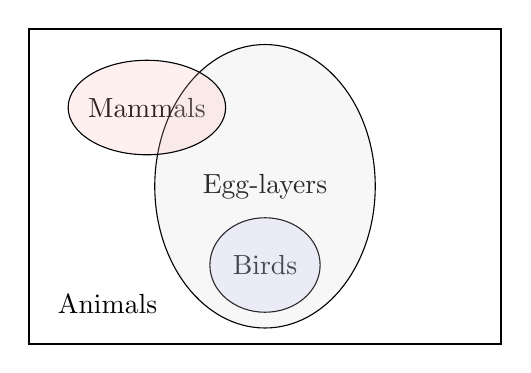
\begin{tikzpicture}
		\draw[thick] (0,0) -- (0,4) -- (6,4) -- (6,0) -- cycle;
		\node (a) at (1,0.5) {Animals};
		\node (e) at (3,2) {Egg-layers};
		\node (b) at (3,1) {Birds};
		\node (m) at (1.5,3) {Mammals};
		\filldraw[fill=blue!30!white, draw =black, fill opacity=0.2] (3,1) ellipse (0.7cm and 0.6cm);
		\filldraw[fill=gray!30!white, draw =black, fill opacity=0.2] (3,2) ellipse (1.4cm and 1.8cm);
		\filldraw[fill=red!30!white, draw =black, fill opacity=0.2] (1.5,3) ellipse (1cm and 0.6cm);
	\end{tikzpicture}
\end{center} In this diagram, the egg-layers are a subset of the animals – not all animals reproduce by laying eggs, so they do not coincide with the whole domain. The birds are a subset of animals too, and in fact wholly within the egg-layers: all birds reproduce oviparously. The mammals are a subset of the animals, and one that overlaps with the egg-layers (the monotremes!), though neither is contained in the other, so the regions overlap without either being wholly within the other. The birds and mammals do not have any common members, so the associated regions do not overlap at all. Note that the sizes of the regions may, but need not, represent the number of things within them. In this diagram they probably don't.

Another example. Consider this interpretation, discussed earlier on page \pageref{poison}: 
		\begin{ekey}
		\item[\text{domain}] people and plants
		\item[C] \gap{1} is a cowboy
		\item[S] \gap{1} sings a sad, sad song
		\item[R] \gap{1} is a rose
		\item[T] \gap{1} has a thorn
	\end{ekey}
The wisdom of Bret Michaels then tells us that the Euler diagram should look like this: \begin{center}
	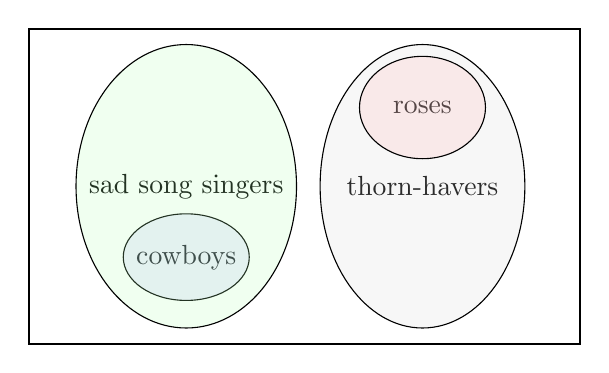
\begin{tikzpicture}
		\draw[thick] (0,0) -- (0,4) -- (7,4) -- (7,0) -- cycle;
		\node (s) at (2,2) {sad song singers};
		\node (t) at (5,2) {thorn-havers};
		\node (c) at (2,1.1) {cowboys};
		\node (r) at (5,3) {roses};
		\filldraw[fill=blue!30!white, draw =black, fill opacity=0.2] (2,1.1) ellipse (0.8cm and 0.55cm);
		\filldraw[fill=green!30!white, draw =black, fill opacity=0.2] (2,2) ellipse (1.4cm and 1.8cm);
		\filldraw[fill=gray!30!white, draw =black, fill opacity=0.2] (5,2) ellipse (1.3cm and 1.8cm);
		\filldraw[fill=red!30!white, draw =black, fill opacity=0.2] (5,3) ellipse (0.8cm and 0.65cm);
	\end{tikzpicture}
\end{center}

If you would like a real challenge, you might try to figure out the interpretation of this Euler diagram from xkcd (`Chat Systems', \url{https://xkcd.com/1810/}):
\begin{center}
	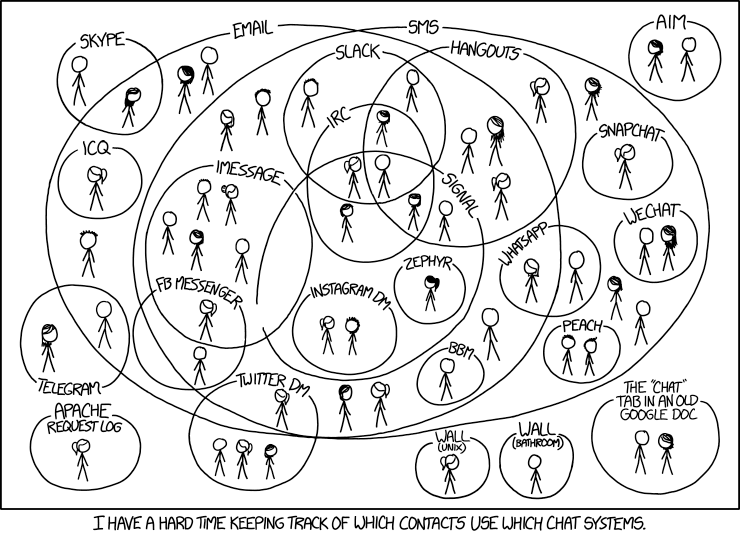
\includegraphics[width=0.85\textwidth]{chat_systems.png}
\end{center}

\paragraph{Representing Two-Place Predicates: Directed Graphs}

Suppose we want to consider just a single two-place predicate, `$R$'. Then we can represent it, in some cases, by depicting the members of the domain by writing them down, and drawing a single-headed arrow between items just in case the relation holds between them (in the right order). Such a diagram is known as a \define{directed graph}, which is given by a collection of \emph{nodes} (the objects in the domain we are representing) and a collection of arrows between them (which represent how the relation holds on that domain.) We stipulate that `$R$' is to hold of \meta{x} and \meta{y} just in case there is an arrow running from \meta{x} to \meta{y} in our diagram. As an example, consider the following interpretation, written in the more standard manner:
\begin{ekey}
	\item[\text{domain}] $1, 2, 3, 4$
	\item[R] \ntuple{1, 2}, \ntuple{2, 3}, \ntuple{3, 4}, \ntuple{4, 1}, \ntuple{1, 3}.
\end{ekey}
That is, an interpretation whose domain is the first four positive whole numbers, and which interprets `$R$' as being true of and only of the specified pairs of numbers. This might be represented by the following simple graph:
\begin{center}
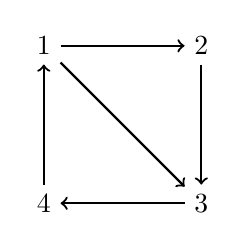
\begin{tikzpicture}
\node (atom1) at (0,2) {1};
\node (atom2) at (2,2) {2};
\node (atom3) at (2,0) {3};
\node (atom4) at (0,0) {4};
\draw[->, thick] (atom1)--(atom2);
\draw[->, thick] (atom2)--(atom3);
\draw[->, thick] (atom3)--(atom4);
\draw[->, thick] (atom4)--(atom1);
\draw[->, thick] (atom1) -- (atom3);
\end{tikzpicture}
\end{center}

Another example; consider the following interpretation: \begin{ekey}
	\item[\text{domain}] $1, 2, 3, 4$
	\item[R] \ntuple{1, 3}, \ntuple{3, 1}, \ntuple{3, 4}, \ntuple{1, 1},\ntuple{3, 3}.
\end{ekey} We might offer this graph to represent it:
\begin{center}
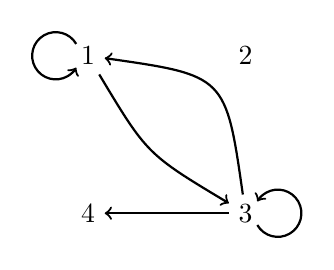
\begin{tikzpicture}
\node (atom1) at (0,2) {1};
\node (atom2) at (2,2) {2};
\node (atom3) at (2,0) {3};
\node (atom4) at (0,0) {4};
\draw[->, thick] (atom3)--(atom4);
\draw[->, thick] (atom1)+(-0.15,0.15) arc (-330:-30:.3); 
\draw[->, thick] (atom3)+(0.15,-0.15) arc (-150:150:.3); 
\draw[->, thick] (atom1) .. controls (0.75,0.75) .. (atom3);
\draw[->, thick] (atom3) .. controls (1.75,1.75) .. (atom1);
\end{tikzpicture}
\end{center} Notice that 2 is in the domain, and hence included as a node in the graph, but it has no arrows attached to it, because it is not included in the relation assigned to $R$. 


If we wanted, we could make our diagrams more complex. For example, we could introduce another kind of arrow to represent an additional two-place relation. Or, we could add names as labels attached to particular objects. Or, to symbolise the extension of a one-place predicate, we might simply draw a ring around some particular objects and stipulate that the thus encircled objects (and only them) are to fall under the predicate `$H$', say.  

Consider how we we might graphically represent the following interpretation, which will make use of all these graphical innovations: \begin{ekey}
	\item[\text{domain}] $2,3,4,5,6$
	\item[G] $\gap{1} \geqslant 4$. 
	\item[D] \gap{1} is distinct from and exactly divisible by \gap{2};
	\item[T] $\gap{1} + 3 = \gap{2}$;
	\item[f] $4$;
\end{ekey} 
This graph represents that interpretation, where the label `$f$' represents the name attached to 4, the blue dotted arrow represents the relation assigned to $T$, the black solid arrow represents the relation assigned to $D$, and the grey ellipse represents the collection of things in the domain which have the property assigned to $G$:
\begin{center}
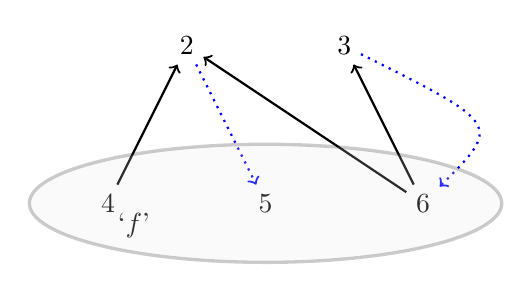
\begin{tikzpicture}
\node (atom2) at (1,2) {2};
\node (atom3) at (3,2) {3};
\coordinate[label=below right:`$f$'] (atom4) at (0,0);
\node (atom4) at (0,0) {4};
\node (atom5) at (2,0) {5};
\node (atom6) at (4,0) {6};
\draw[->, thick] (atom6) -- (atom2);
\draw[->, thick] (atom6) -- (atom3);
\draw[->, thick] (atom4) -- (atom2);
\draw[->, blue, thick, dotted] (atom2) -- (atom5);
\draw[->, blue, thick, dotted] (atom3) .. controls (5,1) .. (atom6);
\filldraw[fill=gray!20!white, draw =black, very thick, opacity=0.2] (2,0) ellipse (3cm and 0.75cm);
\end{tikzpicture}
\end{center}




\keyideas{
	\item An interpretation of \FOL\ is a temporary assignment of extensions to some of the non-logical vocabulary of \FOL\, i.e., the names and predicates of the language.
	\item The extension of a name is a thing from some specified domain.
	\item The extension of an $n$-place predicate is a collection of ordered sequences of length $n$ of things from the domain. The identity predicate has a privileged extension; it is always the collection of pairs from the domain consisting of things and themselves.
	\item The extension of a $0$-place predicate is a truth value; these correspond to atomic sentences of \TFL. 
	\item Given a domain, it is often possible to represent the interpretation of a predicate by means of an Euler diagram or a directed graph on that domain.
}


\practiceproblems
\problempart
Since \FOL\ is an extensional language, if let the \FOL\ name `$s$' denote Superman, and the name `$c$' denote Clark Kent, then `$s=c$' will be true. But it will be true for the same reason that `$s=s$' is true: because \ntuple{Clark Kent,Clark Kent} is in the extension of `$=$'. Can you use this observation as the basis for any argument that English is not an extensional language?

\problempart
Using some of the methods introduced in this section, give a graphical representation of the following interpretations. You will need to rely on your general knowledge to prepare these diagrams. \begin{earg}
	\item \begin{ekey}
		\item[\text{domain}] people
		\item[M] \gap{1} is a musician;
		\item[W] \gap{1} is a woman;
		\item[E] \gap{1} is an economist.
	\end{ekey}
	\item \begin{ekey}
\item[\text{domain}] cards in a standard deck
\item[S] \gap{1} is a seven;
\item[F] \gap{1} is a face card;
\item[R] \gap{1} is red;
\item[j] the Jack of Hearts.
	\end{ekey}
	\item \begin{ekey}
		\item[\text{domain}] Australian states
		\item[L] \gap{1} is larger in population than \gap{2};
		\item[V] \gap{1}'s name ends in a vowel;
		\item[a] South Australia;
		\item[q] Queensland.
	\end{ekey}
\end{earg}

\chapter{Truth in \textnormal{\FOL}}\label{s:TruthFOL}
We know what interpretations are. Since, among other things, they tell us which predicates are true of which objects, they will provide us with an account of the truth of atomic sentences. But we must also present a detailed account of what it is for an arbitrary \FOL\ sentence to be true or false in an interpretation. 

We know from §\ref{s:FOLSentences} that there are three kinds of sentence in \FOL: 
	\begin{itemize}
		\item atomic sentences (i.e., atomic formulae of \FOL\ which have no free variables);
		\item sentences whose main connective is a sentential connective; and
		\item sentences whose main connective is a quantifier.
	\end{itemize}
We need to explain truth for all three kinds of sentence.

I shall offer a completely general explanation in this section. However, to try to keep the explanation comprehensible, I shall at several points use the following interpretation:
	\begin{ekey}
		\item[\text{domain}] all people born before 2000\textsc{ce}
		\item[a] Aristotle
		\item[b] Bush
		\item[W] \gap{1} is wise
		\item[R] \gap{1} was born before \gap{2}
	\end{ekey}
This will be my \emph{go-to example} in what follows.

\section{Atomic sentences}\label{fol.truth.atom}
The truth of atomic sentences should be fairly straightforward. The sentence `$Wa$' should be true just in case `$W$' is true of `$a$'. Given our go-to interpretation, this is true iff Aristotle is wise. Aristotle is wise. So the sentence is true. Equally, `$Wb$' is false on our go-to interpretation.

Likewise, on this interpretation, `$Rab$' is true iff the object named by `$a$' was born before the object named by `$b$'. Well, Aristotle was born before Bush. So `$Rab$' is true. Equally, `$Raa$' is false: Aristotle was not born before Aristotle. 

Dealing with atomic sentences, then, is very intuitive. When $\meta{R}$ is an $n$-place predicate and $\meta{a}_{1}, \meta{a}_{2}, …, \meta{a}_{n}$ are names (not necessarily all different from each other), 

	\factoidbox{
		$\meta{R}\meta{a}_{1}\meta{a}_{2}…\meta{a}_{n}$ is true in an interpretation \textbf{iff}\\
		the objects assigned as the extensions of $\meta{a}_{1}, \meta{a}_{2}, …, \meta{a}_{n}$ in that interpretation (considered in that order) are in the extension assigned to $\meta{R}$ in that interpretation.
	} 

Two other kinds of atomic sentences exist: zero-place predicates, and identity sentences.

\begin{itemize}
	\item A $0$-place predicate is true in an interpretation iff it is assigned the extension true in that interpretation.

	Here in fact, we are using \TFL\ valuations as constituents of \FOL\ interpretations. (A valuation is what you get when you are only intepreting zero-place predicates; we will want it to turn out that the part of \FOL\ which deals just with $0$-place predicates and their truth-functional combinations is the familiar language \TFL, so those interpretations will have to behave like the valuations we are familiar with.)
		\item Identity sentences (two names flanking the identity predicate) are also easy to handle. Where \meta{a} and \meta{b} are any names, 
	\factoidbox{
		$\meta{a} = \meta{b}$ is true in an interpretation \textbf{iff}\\
		 \meta{a} and \meta{b} have the same extension (are assigned the very same object) in that interpretation.}
So in our go-to interpretation, `$a = b$' is false, since Aristotle is distinct from Bush; but `$a=a$' is true.
\end{itemize}






\section{Sentential connectives}\label{fol.truth.sent}
We saw in §\ref{s:FOLSentences} that \FOL\ sentences can be built up from simpler ones using the truth-functional connectives that were familiar from \TFL. The rules governing these truth-functional connectives are \emph{exactly} the same as they were when we considered \TFL. Here they are:
	\factoidbox{Where \meta{A} and \meta{B} are any sentences of \FOL, \begin{itemize}
		\item 
		$\meta{A} \eand \meta{B}$ is true in an interpretation \textbf{iff}\\ both $\meta{A}$ is true and $\meta{B}$ is true in that interpretation
		\item 	$\meta{A} \eor \meta{B}$ is true in an interpretation \textbf{iff}\\ either $\meta{A}$ is true or $\meta{B}$ is true in that interpretation
\item 	$\enot \meta{A}$ is true in an interpretation \textbf{iff} \\$\meta{A}$ is false in that interpretation
\item $\meta{A} \eif \meta{B}$ is true in an interpretation \textbf{iff}\\ either $\meta{A}$ is false or $\meta{B}$ is true in that interpretation
\item $\meta{A} \eiff \meta{B}$ is true in an interpretation \textbf{iff} \\$\meta{A}$ has the same truth value as $\meta{B}$ in that interpretation
	\end{itemize}}
This presents the very same information as the schematic truth tables for the connectives; it just does it in a slightly different way. Some examples will probably help to illustrate the idea. On our go-to interpretation:
	\begin{itemize}
		\item `$a = a \eand Wa$' is true
		\item `$Rab \eand Wb$' is false because, although `$Rab$' is true, `$Wb$' is false
		\item `$a = b \eor Wa$' is true
		\item `$\enot a = b$' is true
		\item `$Wa \eand \enot( a= b \eand Rab)$' is true, because `$Wa$' is true and `$a = b$' is false
	\end{itemize}
Make sure you understand these examples.

\section{When the main connective is a quantifier}\label{fol.truth.quant}
The exciting innovation in \FOL, though, is the use of \emph{quantifiers}. And in fact, expressing the truth conditions for quantified sentences is a bit more fiddly than one might expect. 

Here is a naïve first thought. We want to say that `$\forall x Fx$' is true iff `$F$' is true of everything in the domain. This should not be too problematic: our interpretation will specify directly what `$F$' is true of. 

Unfortunately, this naïve first thought is not general enough. For example, we want to be able to say that `$\forall x \exists y Lxy$' is true just in case `$\exists y Lxy$' is true of everything in the domain. And this is problematic, since our interpretation does not directly specify what `$\exists y Lxy$' is to be true of. Instead, whether or not this is true of something should follow just from the interpretation of `$L$', the domain, and the meanings of the quantifiers. 

So here is a naïve second thought. We might try to say that `$\forall x \exists y Lxy$' is to be true in an interpretation iff $\exists y L\meta{a}y$ is true for \emph{every} name \meta{a} that we have included in our interpretation. And similarly, we might try to say that $\exists y L\meta{a}y$ is true just in case $L\meta{a}\meta{b}$ is true for \emph{some} name \meta{b} that we have included in our interpretation.

Unfortunately, this is not right either. To see this, observe that in our go-to interpretation, we have only given interpretations for \emph{two} names, `$a$' and `$b$'. But the domain – all people born before the year 2000\textsc{ce} – contains many more than two people. I have no intention of trying to name \emph{all} of them!

So here is a third thought. (And this thought is not naïve, but correct.) Although it is not the case that we have named \emph{everyone}, each person \emph{could} have been given a name. So we should focus on this possibility of extending an interpretation, by adding a previously uninterpreted name to our interpretation. I shall offer a few examples of how this might work, centring on our go-to interpretation, and I shall then present the formal definition. 
\begin{itemize}
	\item In our go-to interpretation, `$\exists x Rbx$' should be true. After all, in the domain, there is certainly someone who was born after Bush. Lady Gaga is one of those people. Indeed, if we were to extend our go-to interpretation – temporarily, mind – by adding the name `$c$' to refer to Lady Gaga, then `$Rbc$' would be true on this extended interpretation. And this, surely, should suffice to make `$\exists x Rbx$' true on the original go-to interpretation. 
	\item In our go-to interpretation, `$\exists x (Wx \eand Rxa)$' should also be true. After all, in the domain, there is certainly someone who was both wise and born before Aristotle. Socrates is one such person. Indeed, if we were to extend our go-to interpretation by letting a previously uninterpreted name, `$c$', denote Socrates, then `$Wc \eand Rca$' would be true on this extended interpretation. Again, this should surely suffice to make `$\exists x (Wx \eand Rxa)$' true on the original go-to interpretation. 
	\item In our go-to interpretation, `$\forall x \exists y Rxy$' should be false. After all, consider the last person born in the year 1999. I don't know who that was, but if we were to extend our go-to interpretation by letting a previously uninterpreted name, `$d$', denote that person, then we would not be able to find anyone else in the domain to denote with some further previously uninterpreted name, perhaps `$e$', in such a way that `$Rde$' would be true. Indeed, no matter \emph{whom} we named with `$e$', `$Rde$' would be false. And this observation is surely sufficient to make `$\exists y Rdy$' \emph{false} in our extended interpretation. And this is sufficient to make `$\forall x \exists y Rxy$' false on the original interpretation.
\end{itemize}

If you have understood these three examples, then that's what matters. Strictly speaking, though, we still need to give a precise definition of the truth conditions for quantified sentences. The result, sadly, is a bit ugly, and requires a few new definitions. Brace yourself!

Suppose that \meta{A} is a formula, $\meta{x}$ is a variable, and $\meta{c}$ is a name. We shall write `$\meta{A}\subs{\meta{c}}{\meta{x}}$' to represent the formula that results from replacing or \define{substituting} every free occurrence of $\meta{x}$ in \meta{A} by \meta{c}. So if we began with the formula `$Fxy$', the metalanguage expression ``{`$Fxy$'}$\subs{c}{x}$'' denotes the formula `$Fcy$'. If we began with `$Fyy$', then `$Fyy$'$\subs{c}{x}$ just is the original formula `$Fyy$', since there are no instances of `$x$' in `$Fyy$' to be replaced. If we began with `$Fx \eor \forall x Gx$', then `$Fx \eor \forall x Gx$'$\subs{c}{x}$ is `$Fc \eor \forall x Gx$', since neither occurrence of `$x$' in `$\forall x Gx$' is free.

Suppose we begin with a quantified formula, $\forall \meta{x}\meta{A}$ or $\exists \meta{x}\meta{A}$. If we strip off the quantifier, and pick any name $\meta{c}$, then $\meta{A}\subs{\meta{c}}{\meta{x}}$ is known as a  \define{substitution instance} of the original quantified formulae, and $\meta{c}$ may be called the \define{instantiating name}. So:
	$$\exists x (Rex \eiff Fx)$$
is a substitution instance of 
	$$\forall y \exists x (Ryx \eiff Fx)$$
with the instantiating name `$e$', because  `$\exists x (Ryx \eiff Fx)$'$\subs{e}{y}$ turns out to be `$\exists x (Rex \eiff Fx)$'.

Armed with this notation, the rough idea is as follows. The sentence $\forall \meta{x}\meta{A}$ will be true iff $\meta{A}\subs{\meta{c}}{\meta{x}}$ is true no matter what object (in the domain) we name with $\meta{c}$. Similarly, the sentence $\exists \meta{x}\meta{A}$ will be true iff there is \emph{some} way to assign the name $\meta{c}$ to an object that makes $\meta{A}\subs{\meta{c}}{\meta{x}}$ true. More precisely, we stipulate:\label{quant.tcs.precise}
	\factoidbox{\begin{itemize}
		\item 		$\forall \meta{x}\meta{A}$ is true in an interpretation \textbf{iff}\\ 
		$\meta{A}\subs{\meta{c}}{\meta{x}}$ is true in \emph{every} interpretation that extends the original interpretation by assigning an object to some previously uninterpreted name $\meta{c}$ not appearing in $\meta{A}$ (without changing the original interpretation in any other way).
\item		$\exists \meta{x}\meta{A}$ is true in an interpretation \textbf{iff}\\
		$\meta{A}\subs{\meta{c}}{\meta{x}}$ is true in \emph{some} interpretation that extends the original interpretation by assigning an object to some previously uninterpreted name $\meta{c}$ not appearing in $\meta{A}$ (without changing the original interpretation in any other way).
	\end{itemize}}
That is: we pick a previously uninterpreted name that doesn't appear in \meta{A}.\footnote{There will always be such a previously uninterpreted name: any given sentence of \FOL\ only contains finitely many names, but \FOL\ has a potentially infinite stock of names to draw from.} We uniformly replace any \emph{free} occurrences of the variable \meta{x} in \meta{A} by our previously uninterpreted name, which creates a substitution instance of `$\forall \meta{x}\meta{A}$' and `$\exists \meta{x}\meta{A}$'. Then if this substitution instance is true on every (respectively, some) way of adding an interpretation of the previously uninterpreted name to our existing interpretation, then `$\forall \meta{x}\meta{A}$' (respectively, `$\exists \meta{x}\meta{A}$') is true on that existing interpretation. 

To be clear: all this is doing is formalising (very pedantically) the intuitive idea expressed above. The result is a bit ugly, and the final definition might look a bit opaque. Hopefully, though, the \emph{spirit} of the idea is clear. 

\section{Satisfaction} % Æ introduced this

The discussion of truth in §§\ref{fol.truth.atom}–\ref{fol.truth.quant} only ever involved assigning truth values to sentences. When confronted with formulae involving free variables, we altered them by substituting a previously uninterpreted name for the variable, converting it into a sentence, and temporarily extending the interpretation to cover that previously uninterpreted name. This is a significant departure from the definition of truth for \TFL\ sentences in §\ref{s:SchematicTruthTables}. There, we showed how the truth value of a complex \TFL\ sentence in a valuation depended on the truth value of its constituents in that same valuation. By contrast, on the approach just outlined, the truth value of `$\exists x Fx$' in an interpretation depends on the truth value of some other sentence `$Fc$', which is not a constituent of `$\exists x Fx$', in some different (although related) interpretation! 

There is another way to proceed, which allows arbitrary formulae of \FOL, even those with free variables, to be assigned (temporarily) a truth value. This approach can let the truth value of `$\exists x Fx$' in an interpretation depend on the temporary truth value of `$Fx$' in that same interpretation. This is conceptually  neater than the approach just introduced, and I present it briefly here as an alternative to the substitutional approach of the preceding sections.

\begin{itemize}
 	\item \emph{This section should be regarded as optional, and only for the dedicated student of logic.}
 \end{itemize} 

The inspiration for the approach comes, once again, from thinking of variables in \FOL\ as behaving like pronouns in English. In §\ref{quant.pron} we gave a gloss of `Someone is angry' as `Some person is such that: they are angry'. Concentrate on `they are angry'. This sentence featuring a bare pronoun doesn't express any specific claim intrinsically. But we can, temporarily, fix a referent for the pronoun `they' – temporarily elevating it to the status of a name. If we do so, the sentence can be evaluated. We can introduce a referent by pointing: `They [points to someone] are angry'. Or we can fix a referent by simply assigning one: `Consider that person over there. They are angry'. If we can find someone or other to temporarily be the referent of the pronoun `they', then it will be true that there is someone such that they are angry. If no matter who we fix as the referent, they are angry, then it will be true that everyone is such that they are angry. 

This is, in a nutshell, the idea we will use to handle quantification in \FOL. Let us introduce some terminology: \factoidbox{
	A \define{variable assignment} over an interpretation is an assignment of exactly one object from the domain of that interpretation to each variable that we care to consider.
}  
If we have an interpretation, and a variable assignment, then we can evaluate every formula of \FOL\ – not only sentences. Of course, the evaluation of the open formulae will be very fragile, since even given a single background interpretation, a formula like `$Fx$' might be true relative to one variable assignment and false relative to another. 

Let us start, as before, by giving rules for evaluating atomic formulae of \FOL, given an interpretation and a variable assignment. \factoidbox{Where $\meta{R}$ is any $n$-place predicate ($n ≥ 0$), and $\meta{t}_{1},…,t_{n}$ are any terms – variables or names, then: \begin{itemize}
	\item  $\meta{R}\meta{t}_{1}…\meta{t}_{n}$ is true on a variable assignment over an interpretation \textbf{iff}\\
	$\meta{R}$ is true of the objects assigned to the terms $\meta{t}_{1},…,\meta{t}_{n}$  by that variable assignment and that intepretation, considered in that order.
	\item $\meta{t}_{1}=\meta{t}_{2}$ is true on a variable assignment over an interpretation \textbf{iff}\\
	$\meta{t}_{1}$ and $\meta{t}_{2}$ are assigned the very same object by that variable assignment in that interpretation.
\end{itemize}} These are very similar clauses to those we saw for atomic sentences in §\ref{fol.truth.quant}. Indeed, when we are considering atomic sentences of \FOL, the mention of a variable assignment is redundant, since no atomic sentence contains a variable. (If an atomic formula contains a variable, the variable would be free and the formula thus not a sentence.)

The recursion clauses that extend truth for atomic formulae to truth for arbitrary formulae are these (I omit the clauses for $\eor$, $\eif$, and $\eiff$, which you can easily fill in yourself, following the model in §\ref{fol.truth.sent}): \factoidbox{Where \meta{A} and \meta{B} are formulae of \FOL, and \meta{x} is a variable:
	\begin{itemize}
		\item $\enot \meta{A}$ is true on a variable assignment over an interpretation \textbf{iff}\\
		\meta{A} is false on that variable assignment over that interpretation;
		\item $\meta{A} \eand \meta{B}$ is true on a variable assignment over an interpretation \textbf{iff}\\
		both \meta{A} is true on that variable assignment over that interpretation and \meta{B} is true on that variable assignment over that interpretation;
		\item …
		\item $\forall \meta{x}\meta{A}$ is is true on a variable assignment over an interpretation \textbf{iff}\\
		\meta{A} is true on \emph{every} variable assignment differing from the original one at most in what it assigns to \meta{x} over that interpretation;
		\item $\exists \meta{x}\meta{A}$ is is true on a variable assignment over an interpretation \textbf{iff}\\
		\meta{A} is true on \emph{some} variable assignment differing from the original one at most in what it assigns to \meta{x} over that interpretation.
	\end{itemize}
}

The last two clauses are where this approach is strongest. Rather than considering some substitition instance of $\forall\meta{x}\meta{A}$, we simply consider the direct constituent \meta{A}. Rather than considering all variations on the original interpretation which include some previously uninterpreted name, we simply consider all ways of varying what is assigned to \meta{x} by the original variable assignment, but keeping everything else unchanged. If you see the rationale for the clauses offered in §\ref{fol.truth.quant}, you can see why the clauses just offered are appropriate.

We now have the idea of truth on a variable assignment over an intepretation. But what we want – if this alternative approach is to yield the same end result – is truth in an interpretation. Notice that, given an interpretation, varying the variable assignment can change the truth value of a formula with free variables. But it cannot change the truth value of a formula which is a sentence, so if a sentence is true on one variable assignment over an interpretation, it is true on every variable assignment over that interpretation. So we can reintroduce the notion of truth in an intepretation, like so: \factoidbox{
	 \meta{A} is true in an interpretation \textbf{iff}\\
	 \meta{A} is a sentence of \FOL, and \meta{A} is true on any (or every) variable assignment over that interpretation.
} 

Here's how this works in practice. Suppose we want to figure out whether the sentence `$\forall x \exists y Lxy$' is true on an interpretation which  associates the two-place predicate `$L$' with the relation `\gap{1} is no heavier than \gap{2}', and has as its domain the planets in our solar system. We might reason as follows: \begin{quote}
	\emph{For each way of picking planets to be the values of `$x$' and `$y$', either we pick two different planets, and one is lighter than the other (no two planets have the same mass); or we pick the same planet, and `they' are identical in mass. In either case, we can always find something no heavier than anything we pick. So for any variable assignment to `$x$' over this interpretation,  we can then assign something to `$y$' so as to make `$Lxy$' true on that joint assignment. Hence no matter what we assign to `$x$', `$\exists y Lxy$' is true on that assignment. But since that is true no matter what we assign to `$x$', `$\forall x \exists y Lxy$' is true on every variable assignment over this interpretation. But that latter is a sentence, so is true in this interpretation.}
\end{quote}

Let us say that a sequence of objects \ntuple{$a_{1},…,a_{n}$} \define{satisfies} a formula $\meta{A}$ in which the variables $\meta{x}_{1},…,\meta{x}_{n}$ occur freely iff there is a variable assignment over an intepretation whose domain includes each $a_{i}$, and which assigns each $a_{i}$ to the variable $\meta{x}_{i}$, and on which \meta{A} is true over that interpretation. What we have expressed in terms of variable assignments could have been expressed, a little more awkwardly, using the notion of some objects satisfying a formula. Indeed, this is how Alfred Tarski, the inventor of this approach to truth in \FOL, first introduced the idea.\footnote{A translation of his original 1933 paper is `The Concept of Truth in Formalized Languages', 1983, in Tarski, \emph{Logic, Semantics, Metamathematics}, Indianapolis: Hackett, pp. 152–278. It is rather technical in places.}

\keyideas{
	\item An atomic sentence  of \FOL\ is true in an interpretation iff the extensions of the names occurring in it, taken in the appropriate order, fall in the extension of the predicate they accompany.
	\item A compound sentence  of \FOL\ has truth conditions relative to an interpretation that are the same as those for \TFL, if the main connective is truth-functional.
	\item A compound sentence of \FOL\ whose main connective is a quantifier `$\forall x$' (resp., `$\exists x$') is true in an interpretation if on every (resp., some) interpretation extending the first by assigning an extension to some previously uninterpreted name `$c$', the result of replacing every occurence of the variable `$x$' bound by the quantifier with $c$ is true.
}

\practiceproblems


\problempart
\label{pr.TorF1}
Consider the following interpretation:
	\begin{ekey}
		\item[\text{domain}] The domain comprises only Corwin and Benedict
		\item[A] is to be true of both Corwin and Benedict
		\item[B] is to be true of Benedict only
		\item[N] is to be true of no one
		\item[c] is to refer to Corwin
	\end{ekey}
Determine whether each of the following sentences is true or false in that interpretation:
\begin{earg}
\item $Bc$
\item $Ac \eiff \enot Nc$
\item $Nc \eif (Ac \eor Bc)$
\item $\forall x Ax$
\item $\forall x \enot Bx$
\item $\exists x(Ax \eand Bx)$
\item $\exists x(Ax \eif Nx)$
\item $\forall x(Nx \eor \enot Nx)$
\item $\exists x Bx \eif \forall x Ax$
\end{earg}

\problempart
\label{pr.TorF3}
Consider the following interpretation:	
	\begin{ekey}
		\item[\text{domain}] The domain comprises only Lemmy, Courtney and Eddy
		\item[G] is to be true of Lemmy, Courtney and Eddy.
		\item[H] is to be true of and only of Courtney
		\item[M] is to be true of and only of Lemmy and Eddy
		\item[c] is to refer to Courtney
		\item[e] is to refer to Eddy
	\end{ekey}
Determine whether each of the following sentences is true or false in that interpretation:
\begin{earg}
\item $Hc$
\item $He$
\item $Mc \eor Me$
\item $Gc \eor \enot Gc$
\item $Mc \eif Gc$
\item $\exists x Hx$
\item $\forall x Hx$
\item $\exists x \enot Mx$
\item $\exists x(Hx \eand Gx)$
\item $\exists x(Mx \eand Gx)$
\item $\forall x(Hx \eor Mx)$
\item $\exists x Hx \eand \exists x Mx$
\item $\forall x(Hx \eiff \enot Mx)$
\item $\exists x Gx \eand \exists x \enot Gx$
\item $\forall x\exists y(Gx \eand Hy)$
\end{earg}

\problempart
% \label{pr.TorF3}
Following the diagram conventions introduced at the end of §\ref{s:Interpretations}, consider the following interpretation:	
\begin{center}
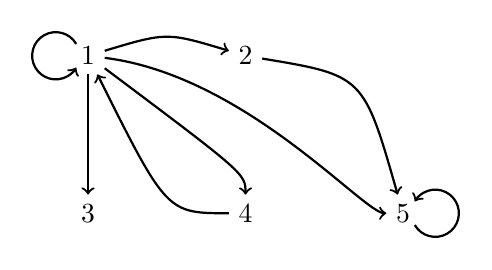
\begin{tikzpicture}
\node (atom1) at (0,2) {1};
\node (atom2) at (2,2) {2};
\node (atom4) at (0,0) {3};
\node (atom5) at (2,0) {4};
\node (atom6) at (4,0) {5};
\draw[->, thick] (atom1)+(-0.15,0.15) arc (-330:-30:.3); 
\draw[->, thick] (atom6)+(0.15,-0.15) arc (-150:150:.3); 
\draw[->, thick] (atom1) .. controls (1,2.3) .. (atom2);
\draw[->, thick] (atom1) -- (atom4);
\draw[->, thick] (atom5) .. controls (1,0) .. (atom1);
\draw[->, thick] (atom1) .. controls (2,0.5) .. (atom5);
\draw[->, thick] (atom1) .. controls (2,1.75) and (3.5,0) .. (atom6);
\draw[->, thick] (atom2) .. controls (3.5,1.75) .. (atom6);
\end{tikzpicture}
\end{center}
Determine whether each of the following sentences is true or false in that interpretation:
\begin{earg}
\item $\exists x Rxx$
\item $\forall x Rxx$
\item $\exists x \forall y Rxy$
\item $\exists x \forall y Ryx$
\item $\forall x \forall y \forall z ((Rxy \eand Ryz) \eif Rxz)$
\item $\forall x \forall y \forall z ((Rxy \eand Rxz) \eif Ryz)$
\item $\exists x \forall y \enot Rxy$
\item $\forall x(\exists y Rxy \eif \exists y Ryx)$
\item $\exists x \exists y (\enot x = y \eand Rxy \eand Ryx)$
\item $\exists x \forall y(Rxy \eiff x = y)$
\item $\exists x \forall y(Ryx \eiff x = y)$
\item $\exists x \exists y(\enot x = y \eand Rxy \eand \forall z(Rzx \eiff y = z))$
\end{earg}

\problempart
Why, when we are trying to figure out whether `$\forall x Rxa$' is true in an interpretation, do we need to consider whether `$Rca$' is true in some expanded interpretation with a \emph{new} name `$c$'. Why can't we make do with substituting a name we've already interpreted?

\problempart
Explain why on page \pageref{quant.tcs.precise} we did not give the truth conditions for the existential quantifer like this: \begin{quote}
	$\exists\meta{x}\meta{A}\subs{x}{c}$ is true in an interpretation $I$ iff in \emph{some} interpretation just like $I$ except that might assign something different to \meta{c}, $\meta{A}$ is true.
\end{quote}






\chapter{Semantic concepts}\label{FOL.semantics}
Offering a precise definition of truth in \FOL\ was more than a little fiddly. But now that we are done, we can define various central logical notions. These will look very similar to the definitions we offered for \TFL. However, remember that they concern \emph{interpretations}, rather than valuations. 


We will use the symbol `$\entails$' for entailment in \FOL, much as we did for \TFL. This introduces an ambiguity, but a harmless one, since every valid argument in \TFL\ remains a valid argument in \FOL.

So:\factoidbox{\begin{itemize}
	\item  	$\meta{A}_1, \meta{A}_2, …, \meta{A}_n$ together \define{entail} \meta{C} (written $\meta{A}_1, \meta{A}_2, …, \meta{A}_n \entails\meta{C}$) iff there is no interpretation in which all of $\meta{A}_1, \meta{A}_2, …, \meta{A}_n$ are true and in which \meta{C} is false.
	\item An \FOL\ sentence $\meta{A}$ is a \define{logical truth} iff $\meta{A}$ is true in every interpretation; this is written  $\entails\meta{A}$.
	\item $\meta{A}$ is a \define{contradiction} iff $\meta{A}$ is false in every interpretation; i.e., $\entails\enot\meta{A}$.

\item Two \FOL\ sentences \meta{A} and \meta{B} are \define{logically equivalent} iff they are true in exactly the same interpretations as each other; i.e., both $\meta{A}\entails\meta{B}$ and $\meta{B}\entails\meta{A}$.
\item The \FOL\ sentences $\meta{A}_1,\meta{A}_2,…, \meta{A}_n$ are \define{jointly consistent} iff there is some interpretation in which all of the sentences are true. They are \define{jointly inconsistent} iff there is no such interpretation.\end{itemize}}

As before, there is a close connection between validity and entailment: \factoidbox{
 $\meta{A}_1, \meta{A}_2, … \meta{A}_n \ttherefore \meta{C}$ is \define{valid} in \FOL\ iff there is no interpretation in which all of the premises are true and the conclusion is false; i.e., $\meta{A}_1,\meta{A}_2,… \meta{A}_n \entails\meta{C}$. It is \define{invalid} in \FOL\ otherwise.} Our entailments are conclusive in virtue of form, because the consideration of many alternative interpretations of the non-logical expressions involved means that no argument can be conclusive because of some special `connection in meaning' between such expressions in the language. Entailment in \FOL\ reflects only the logical structure of the sentences involved, where this now includes the new logical resources of \FOL\ over \TFL.

\section{Some subtleties about truth and interpretation} % Æ added

Our interpretations allow us a precise characterisation of formal truth for \FOL. In §\ref{s:Valid}, we introduced the idea of the structure of a sentence, and the pragmatic approach that logicians take to that notion. In \FOL, the logical constants are those of \TFL\ plus the quantifiers and the identity predicate. But every other item of the language is up for reinterpretation, and our interpretations allow us to reinterpret these expressions in an arbitrary fashion.

In \TFL, we were able to characterise a logical truth as a sentence which is actually true on every reinterpretation of non-logical expressions (in \TFL, the non-logical expressions are just are the atomic sentences). And we characterised a formally valid argument as one in which each possible reinterpretation (i.e., valuation) of the  premises which makes them actually true, is also one which makes the conclusion actually true.

But this account of formal validity needs refining when it comes to \FOL. Consider the \FOL\ sentence which says that there are at least three things: $$\exists x \exists y \exists z (x≠y \eand x≠z \eand y≠z).$$ This sentence contains no non-logical expressions. Hence the sentence has a constant meaning, and is true on each reinterpretation just in case it is actually true. It is actually true – there are actually at least three things. Hence our \TFL-inspired account of logical truth would suggest that this sentence is a logical truth. But it seems very strange to think that it is a truth of logic alone that there are at least three things. Isn't it possible that there had been fewer?

The keen-eyed among you will have noticed that this sentence is not, in fact, a logical truth of \FOL. The reason is that in defining truth for sentences of \FOL, we considered not just reinterpretations of the non-logical expressions, but also we allowed the domain of our interpretation to freely depart from actuality. So we are, in effect, allowing our interpretations to vary the meanings of the non-logical vocabulary \emph{and} to vary the possible situations at which our sentences are to be evaluated. So we can consider a possible situation in which there are just two things, and if that situation provides the domain of an interpretation, there is no way of extending that interpretation to three names `$a$', `$b$', and `$c$' such that `$a≠b \eand a≠c \eand b≠c$' is true; hence `$\exists x \exists y \exists z (x≠y \eand x≠z \eand y≠z)$' isn't true on the original interpretation.

One sentence of this class is nevertheless a logical truth: the claim that something exists, `$\exists x x=x$'. Since it is a constraint on \FOL\ domains that they cannot be empty (§\ref{sec_domains}), there is for any interpretation a way of adding a previously uninterpreted name `$c$' which denotes an object in the domain, and of course `$c=c$' is true in that extended interpretation, since each name must have a referent in any interpretation, and the identity predicate is always interepreted as representing pairs of objects in the domain and themselves.

\keyideas{
	\item Definitions of entailment, consistency, contradiction and logical equivalence can be given for \FOL\ that are very close parallels to those for \TFL, though given in terms of intepretations not valuations.
	\item The notion of a logical truth in \FOL\ is slightly different than the notion of a tautology, since we allow interpretations that vary not just in what they assign as extensions to the non-logical vocabulary, but also variation in the domain over which quantifiers range. Nothing like the latter feature occurs in \TFL\ valuations, but it is crucial for ensuring that contingent truths without names or non-logical predicates aren't misclassified as logical truths.
}





\chapter{Demonstrating Consistency and Invalidity}
\label{sec.UsingModels}

\section{Logical truths and contradictions}
Suppose we want to show that `$\exists xAxx \eif Bd$' is \emph{not} a logical truth. This requires showing that the sentence is not true in every interpretation; i.e.,\ that it is false in some interpretation. If we can provide just one interpretation in which the sentence is false, then we will have shown that the sentence is not a logical truth.

In order for `$\exists xAxx \eif Bd$' to be false, the antecedent (`$\exists x Axx$') must be true, and the consequent (`$Bd$') must be false. To construct such an interpretation, we start by specifying a domain. Keeping the domain small makes it easier to specify what the predicates will be true of, so we shall start with a domain that has just one member. For concreteness, let's say it is the city of Paris. 
	\begin{ekey}
		\item[\text{domain}] Paris
	\end{ekey}
The name `$d$' must name something in the domain, so we have no option but:
	\begin{ekey}
		\item[d] Paris
	\end{ekey}
Recall that we want `$\exists x Axx$' to be true, so we want all members of the domain to be paired with themselves in the extension of `$A$'. We can offer:
	\begin{ekey}
		\item[A] \gap{1} is in the same place as \gap{2}
	\end{ekey}
Now `$Add$' is true, so it is surely true that `$\exists x Axx$'. Next, we want `$Bd$' to be false, so the referent of `$d$' must not be in the extension of `$B$'. We might simply offer:
	\begin{ekey}
		\item[B] \gap{1} is in Germany
	\end{ekey}
Now we have an interpretation where `$\exists x Axx$' is true, but where `$Bd$' is false. So there is an interpretation where `$\exists x Axx \eif Bd$' is false. So `$\exists x Axx \eif Bd$' is not a logical truth.

We can just as easily show that `$\exists xAxx \eif Bd$' is not a contradiction. We need only specify an interpretation in which `$\exists xAxx \eif Bd$' is true; i.e., an interpretation in which either `$\exists x Axx$' is false or `$Bd$' is true. Here is one:
	\begin{ekey}
		\item[\text{domain}] Paris
		\item[d] Paris
		\item[A] \gap{1} is in the same place as \gap{2}
		\item[B] \gap{1} is in France
	\end{ekey}
This shows that there is an interpretation where `$\exists xAxx \eif Bd$' is true. So `$\exists x Axx \eif Bd$' is not a contradiction.

\section{Logical equivalence}
Suppose we want to show that `$\forall x Sx$' and `$\exists x Sx$' are not logically equivalent. We need to construct an interpretation in which the two sentences have different truth values; we want one of them to be true and the other to be false. We start by specifying a domain. Again, we make the domain small so that we can specify extensions easily. In this case, we shall need at least two objects. (If we chose a domain with only one member, the two sentences would end up with the same truth value. In order to see why, try constructing some partial interpretations with one-member domains.) For concreteness, let's take:
	\begin{ekey}
		\item[\text{domain}] Ornette Coleman, Sarah Vaughan
	\end{ekey}
We can make `$\exists x Sx$' true by including something in the extension of `$S$', and we can make `$\forall x Sx$' false by leaving something out of the extension of `$S$'. For concreteness we shall offer:
	\begin{ekey}
		\item[S] \gap{1} plays saxophone
	\end{ekey}
Now `$\exists x Sx$' is true, because `$S$' is true of Ornette Coleman. Slightly more precisely, extend our interpretation by allowing `$c$' to name Ornette Coleman.  `$Sc$' is true in this extended interpretation, so `$\exists x Sx$' was true in the original interpretation. Similarly, `$\forall x Sx$' is false, because `$S$' is false of Sarah Vaughan. Slightly more precisely, extend our interpretation by allowing `$d$' to name Sarah Vaughan, and `$Sd$' is false in this extended interpretation, so `$\forall x Sx$' was false in the original interpretation. We have provided a counter-interpretation to the claim that `$\forall x Sx$' and `$\exists x Sx$' are logically equivalent.
	\factoidbox{
		To show that $\meta{A}$ is not a logical truth, it suffices to find an interpretation where $\meta{A}$ is false.
		
		To show that $\meta{A}$ is not a contradiction, it suffices to find an interpretation where $\meta{A}$ is true.
		
		To show that $\meta{A}$ and $\meta{B}$ are not logically equivalent, it suffices to find an interpretation where one is true and the other is false.
	}

\section{Validity, entailment and consistency}
To test for validity, entailment, or consistency, we typically need to produce interpretations that determine the truth value of several sentences simultaneously. 

Consider the following argument in \FOL:
$$\exists x(Gx \eif Ga) \ttherefore \exists x Gx \eif Ga$$
To show that this is invalid, we must make the premise true and the conclusion false. The conclusion is a conditional, so to make it false, the antecedent must be true and the consequent must be false. Clearly, our domain must contain two objects. Let's try:
	\begin{ekey}
		\item[\text{domain}] Karl Marx, Ludwig von Mises
		\item[G] \gap{1} hated communism
		\item[a] Karl Marx
	\end{ekey}
Given that Marx wrote \emph{The Communist Manifesto}, `$Ga$' is plainly false in this interpretation. But von Mises famously hated communism. So `$\exists x Gx$' is true in this interpretation. Hence `$\exists x Gx \eif Ga$' is false, as required. 

But does this interpretation make the premise true? Yes it does! For `$\exists x (Gx \eif Ga)$' to be true,  `$Gc \eif Ga$' must be true in  some extended interpretation that is almost exactly like the interpretation just given, except that it also interprets some previously uninterpreted name `$c$'. Let's extend our original interpretation by letting `$c$' denote Karl Marx – the same thing as `$a$' denotes in the original interpretation. Since `$a$' and `$c$' denote the same thing in the extended interpretation, obviously `$Gc \eif Ga$' will be true. So `$\exists x (Gx \eif Ga)$' is true in the original interpretation. So the premise is true, and the conclusion is false, in this original interpretation. The argument is therefore invalid. 

In passing, note that we have also shown that `$\exists x(Gx \eif Ga)$' does \emph{not} entail `$\exists x Gx \eif Ga$'. And equally, we have shown that the sentences `$\exists x (Gx \eif Ga)$' and `$\enot (\exists x Gx \eif Ga)$' are jointly consistent.

Let's consider a second example. Consider:
	$$\forall x \exists y Lxy \ttherefore \exists y \forall x Lxy$$
Again, I want to show that this is invalid. To do this, we must make the premises true and the conclusion false. Here is a suggestion:
	\begin{ekey}
		\item[\text{domain}] People with a living biological sibling
		\item[L] \gap{1} shares a parent with \gap{2}
	\end{ekey}
The premise is clearly true on this interpretation. Anyone in the domain has a living sibling. That sibling will also, then, be in the domain, because one cannot be someone's sibling without also having  them as a sibling. So for everyone in the domain, there will be at least one other person in the domain who is their sibling, and thus has a parent in common with them. Hence `$\forall x \exists y Lxy$' is true. But the conclusion is clearly false, for that would require that there is some single person who shares a parent with everyone in the domain, and there is no such person. So the argument is invalid. We observe immediately that the sentences `$\forall x \exists y Lxy$' and `$\enot\exists y \forall x Lxy$' are jointly consistent and that `$\forall x \exists y Lxy$' does not entail `$\exists y \forall x Lxy$'. 

For my third example, I shall mix things up a bit. In §\ref{s:Interpretations}, I described how we can present some interpretations using diagrams. For example:
\begin{center}
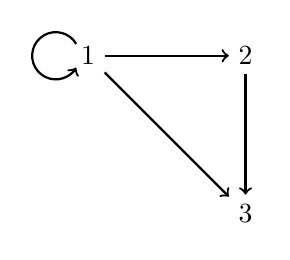
\begin{tikzpicture}
\node (atom1) at (0,2) {1};
\node (atom2) at (2,2) {2};
\node (atom3) at (2,0) {3};
\draw[->, thick] (atom1)--(atom2);
\draw[->, thick] (atom1)--(atom3);
\draw[->, thick] (atom1)+(-0.15,0.15) arc (-330:-30:.3); 
\draw[->, thick] (atom2) -- (atom3);
\end{tikzpicture}
\end{center}
Using the conventions employed in §\ref{s:Interpretations}, the domain of this interpretation is the first three positive whole numbers, and `$R$' is true of \meta{x} and \meta{y} just in case there is an arrow from \meta{x} to \meta{y} in our diagram. Here are some sentences that the interpretation makes true:
	\begin{itemize}
		\item `$\forall x \exists y Ryx$' 
		\item `$\exists x \forall y Rxy$' \hfill witness 1
		\item `$\exists x \forall y (Ryx \eiff x = y)$' \hfill witness 1
		\item `$\exists x \exists y \exists z (\enot y = z \eand Rxy \eand Rzx)$' \hfill witness 2
		\item `$\exists x \forall y \enot Rxy$' \hfill witness 3
		\item `$\exists x (\exists y Ryx \eand \enot \exists y Rxy)$' \hfill witness 3
	\end{itemize}
This immediately shows that all of the preceding six sentences are jointly consistent. We can use this observation to generate \emph{invalid} arguments, e.g.:
	\begin{align*}
		\forall x \exists y Ryx, \exists x \forall y Rxy  &\ttherefore  \forall x \exists y Rxy\\
		\exists x \forall y Rxy, \exists x \forall y \enot Rxy & \ttherefore \enot \exists x \exists y \exists z (\enot y = z \eand Rxy \eand Rzx)
	\end{align*}
and many more besides.

	\factoidbox{
	To show that $\meta{A}_1, \meta{A}_2, …, \meta{A}_n \ttherefore \meta{C}$ is invalid, it suffices to find an interpretation where all of $\meta{A}_1, \meta{A}_2, …, \meta{A}_n$ are true and where $\meta{C}$ is false.
	
	That same interpretation will show that $\meta{A}_1, \meta{A}_2, …, \meta{A}_n$ do not entail $\meta{C}$.
	
	That same interpretation will show that $\meta{A}_1, \meta{A}_2, …, \meta{A}_n, \enot \meta{C}$ are jointly consistent.}
When you provide an interpretation to refute a claim – to logical truth, say, or to entailment – this is sometimes called providing a \emph{counter-interpretation} (or providing a \emph{counter-model}).

\keyideas{
	\item Testing for consistency and invalidity involves displaying just a single appropriate interpretation.
	\item It can be a subtle matter to figure out what such an interpretation might be like. 
	\item An interpretation which shows an argument invalid is a counterexample to that argument. 
}

\practiceproblems

\problempart
The following entailments are correct in \FOL. In each case, explain why.
\begin{earg}
 	\item $\forall x Qx, \forall x (Qx \eif Rx) \entails \exists x Rx$;
 	\item $\forall x\forall y \bigl(Rxy \eif \forall z(Ryz \eif x≠z)\bigr) \entails (Raa \eif \enot Raa)$.
 \end{earg} 

\problempart
\label{pr.Contingent}
Show that each of the following is neither a logical truth nor a contradiction:
\begin{earg}
\item \leftsolutions\ $Da \eand Db$
\item \leftsolutions\ $\exists x Txh$
\item \leftsolutions\ $Pm \eand \enot\forall x Px$
\item $\forall z Jz \eiff \exists y Jy$
\item $\forall x (Wxmn \eor \exists yLxy)$
\item $\exists x (Gx \eif \forall y My)$
\item $\exists x (x = h \eand x = i)$
\end{earg}

\solutions
\problempart
\label{pr.NotEquiv}
Show that the following pairs of sentences are not logically equivalent.
\begin{earg}
\item $Ja$, $Ka$
\item $\exists x Jx$, $Jm$
\item $\forall x Rxx$, $\exists x Rxx$
\item $\exists x Px \eif Qc$, $\exists x (Px \eif Qc)$
\item $\forall x(Px \eif \enot Qx)$, $\exists x(Px \eand \enot Qx)$
\item $\exists x(Px \eand Qx)$, $\exists x(Px \eif Qx)$
\item $\forall x(Px\eif Qx)$, $\forall x(Px \eand Qx)$
\item $\forall x\exists y Rxy$, $\exists x\forall y Rxy$
\item $\forall x\exists y Rxy$, $\forall x\exists y Ryx$
\end{earg}



\problempart
Show that the following sentences are jointly consistent:
\begin{earg}
\item $Ma, \enot Na, Pa, \enot Qa$
\item $Lee, Leg, \enot Lge, \enot Lgg$
\item $\enot (Ma \eand \exists x Ax), Ma \eor Fa, \forall x(Fx \eif Ax)$
\item $Ma \eor Mb, Ma \eif \forall x \enot Mx$
\item $\forall y Gy, \forall x (Gx \eif Hx), \exists y \enot Iy$
\item $\exists x(Bx \eor Ax), \forall x \enot Cx, \forall x\bigl( (Ax \eand Bx) \eif Cx\bigr)$
\item $\exists x Xx, \exists x Yx, \forall x(Xx \eiff \enot Yx)$
\item $\forall x(Px \eor Qx), \exists x\enot(Qx \eand Px)$
\item $\exists z(Nz \eand Ozz), \forall x\forall y(Oxy \eif Oyx)$
\item $\enot \exists x \forall y Rxy, \forall x \exists y Rxy$
\item $\enot Raa$, $\forall x (x=a \eor Rxa)$
\item $\forall x\forall y\forall z(x=y \eor y=z \eor x=z)$, $\exists x\exists y\ \enot x= y$
\item $\exists x\exists y(Zx \eand Zy \eand x=y)$, $\enot Zd$, $d=e$
\end{earg}

\problempart
Show that the following arguments are invalid:
\begin{earg}
\item $\forall x(Ax \eif Bx) \ttherefore \exists x Bx$
\item $\forall x(Rx \eif Dx), \forall x(Rx \eif Fx) \ttherefore \exists x(Dx \eand Fx)$
\item $\exists x(Px\eif Qx) \ttherefore \exists x Px$
\item $Na \eand Nb \eand Nc \ttherefore \forall x Nx$
\item $Rde, \exists x Rxd \ttherefore Red$
\item $\exists x(Ex \eand Fx), \exists x Fx \eif \exists x Gx \ttherefore \exists x(Ex \eand Gx)$
\item $\forall x Oxc, \forall x Ocx \ttherefore \forall x Oxx$
\item $\exists x(Jx \eand Kx), \exists x \enot Kx, \exists x \enot Jx \ttherefore \exists x(\enot Jx \eand \enot Kx)$
\item $Lab \eif \forall x Lxb, \exists x Lxb \ttherefore Lbb$
\item $\forall x(Dx \eif \exists y Tyx) \ttherefore \exists y \exists z\ \enot y= z$
\end{earg}

\chapter{Reasoning about all interpretations: demonstrating inconsistency and validity}

\section{Logical truths and contradictions}
We can show that a sentence is \emph{not} a logical truth just by providing one carefully specified interpretation: an interpretation in which the sentence is false. To show that something is a logical truth, on the other hand, it would not be enough to construct ten, one hundred, or even a thousand interpretations in which the sentence is true. A sentence is only a logical truth if it is true in \emph{every} interpretation, and there are infinitely many interpretations. We need to reason about all of them, and we cannot do this by dealing with them one by one!

Sometimes, we can reason about all interpretations fairly easily. For example, we can offer a relatively simple argument that `$Raa\eiff Raa$' is a logical truth:
	\begin{quote}
		\label{allmodels1}
		Any relevant interpretation will give `$Raa$' a truth value. If `$Raa$' is true in an interpretation, then `$Raa \eiff Raa$' is true in that interpretation. If `$Raa$' is false in an interpretation, then `$Raa \eiff Raa$' is true in that interpretation. These are the only alternatives. So `$Raa \eiff Raa$' is true in every interpretation. Therefore, it is a logical truth.
	\end{quote}
This argument is valid, of course, and its conclusion is true. However, it is not an argument in \FOL. Rather, it is an argument in English \emph{about} \FOL: it is an argument in the metalanguage. 

Note another feature of the argument. Since the sentence in question contained no quantifiers, we did not need to think about how to interpret `$a$' and `$R$'; the point was just that, however we interpreted them, `$Raa$' would have some truth value or other. (We could ultimately have given the same argument concerning \TFL\ sentences.)

Here is another bit of reasoning. Consider the sentence `$\forall x(Rxx\eiff Rxx)$'. Again, it should obviously be a logical truth. But to say precisely why is quite a challenge. We cannot say that `$Rxx \eiff Rxx$' is true in every interpretation, since `$Rxx \eiff Rxx$' is not even a \emph{sentence} of \FOL\ (remember that `$x$' is a variable, not a name). So we have to be a bit cleverer. 
	\begin{quote}
		Consider some arbitrary interpretation. Consider some arbitrary member of the model's domain, which, for convenience, we shall call \emph{obbie}, and suppose we extend our original interpretation by adding a previously uninterpreted name, `$c$', to name \emph{obbie}. Then either `$Rcc$' will be true or it will be false. If `$Rcc$' is true, then `$Rcc \eiff Rcc$' is true. If `$Rcc$' is false, then `$Rcc \eiff Rcc$' will be true. So either way, `$Rcc \eiff Rcc$' is true. Since there was nothing special about \emph{obbie} – we might have chosen any object – we see that no matter how we extend our original interpretation by allowing `$c$' to name some new object, `$Rcc \eiff Rcc$' will be true in the new interpretation. So `$\forall x (Rxx \eiff Rxx)$' was true in the original interpretation. But we chose our interpretation arbitrarily. So `$\forall x (Rxx \eiff Rxx)$' is true in every interpretation. It is therefore a logical truth.
	\end{quote}
This is quite longwinded, but, as things stand, there is no alternative. In order to show that a sentence is a logical truth, we must reason about \emph{all} interpretations. 

But sometimes we can draw a conclusion about some way all interpretations must be, by considering a hypothetical interpretation which isn't that way, and showing that hypothesis leads to trouble. Here is an example. \begin{quote}
	Suppose there were an interpretation which makes `$a≠b \eif \enot \exists x(x=a \eand x=b)$' false. Then while `$a≠b$' is true on that interpretation, `$\enot \exists x(x=a \eand x=b)$' must be false. So `$\exists x(x=a \eand x=b)$' must be true; and hence it has some true substitition instance with some previously uninterpreted name `$c$' as the instantiating name: `$c=a \eand c=b$' is true. But then it must also be that `$a=b$' is true, which contradicts our original supposition that `$a≠b$' is true on this intepretation. So there can be no such interpretation, and hence the sentence cannot be false on any interpretation and must be a logical truth.
\end{quote} This is an example of \define{\emph{reductio}} reasoning\label{reductio}: we assume something, and derive some absurdity or contradiction; we then conclude that our assumption is to be rejected. It is often easier to show that all Fs have a property by deriving an absurdity from the assumption that some F lacks the property, than it is to show it `directly' by considering each F in turn. This is a powerful technique, used widely in mathematics and elsewhere.

\section{Other cases}
Similar points hold of other cases too. Thus, we must reason about all interpretations if we want to show:
	\begin{itemize}
		\item that a sentence is a contradiction; for this requires that it is false in \emph{every} interpretation. 
		\item that two sentences are logically equivalent; for this requires that they have the same truth value in \emph{every} interpretation.
		\item that some sentences are jointly inconsistent; for this requires that there is no interpretation in which all of those sentences are true together; i.e., that, in \emph{every} interpretation, at  least one of those sentences is false.
		\item that an argument is valid; for this requires that the conclusion is true in \emph{every} interpretation where the premises are true. 
		\item that some sentences entail another sentence.
	\end{itemize}
The problem is that, with the tools available to you so far, reasoning about all interpretations is a serious challenge! Let's take just one more example. Here is an argument which is obviously valid:
	$$\forall x(Hx \eand Jx) \ttherefore \forall x Hx$$
After all, if everything is both H and J, then everything is H. But we can only show that the argument is valid by considering what must be true in every interpretation in which the premise is true. And to show this, we would have to reason as follows:
	\begin{quote}
		Consider an arbitrary interpretation in which the premise `$\forall x(Hx \eand Jx)$' is true. It follows that, however we expand the interpretation with a previously uninterpreted name, for example `$c$', `$Hc \eand Jc$' will be true in this new interpretation. `$Hc$' will, then, also be true in this new interpretation. But since this held for \emph{any} way of expanding the interpretation, it must be that `$\forall x Hx$' is true in the old interpretation. And we assumed nothing about the interpretation except that it was one in which `$\forall x(Hx \eand Jx)$'  is true. So any interpretation in which `$\forall x(Hx \eand Jx)$' is true is one in which `$\forall x Hx$' is true. The argument is valid!
\end{quote}
Even for a simple argument like this one, the reasoning is somewhat complicated. For longer arguments, the reasoning can be extremely torturous.

\emph{Reductio} reasoning is particularly useful in demonstrating the validity of valid arguments. In that case we will typically make the hypothetical supposition that there is some interpretation which makes the premises true and the conclusion false, and then derive an absurdity from that supposition. From that we can conclude there is no such intepretation, and hence that any interpretation which makes the premises true must also be one which makes the conclusion true. 

The following table summarises whether a single (counter-)interpretation suffices, or whether we must reason about all interpretations (whether directly considering them all, or indirectly making use of \emph{reductio}).


\begin{center}
\begin{tabular}{l l l} \toprule 
%\cline{2-3}
 & \textbf{Yes} & \textbf{No}\\
 \midrule
%\cline{2-3}
logical truth? & all interpretations & one counter-interpretation\\
contradiction? &  all interpretations  & one counter-interpretation\\
equivalent? & all interpretations & one counter-interpretation\\
consistent? & one interpretation & consider all interpretations\\
valid? & all interpretations & one counter-interpretation\\
entailment? & all interpretations & one counter-interpretation\\
\bottomrule \end{tabular}
\end{center}
\label{table.ModelOrArgument}
This might usefully be compared with the table at the end of §\ref{s:directPartialTruthTable}. The key difference resides in the fact that \TFL\ concerns truth tables, whereas \FOL\ concerns interpretations. This difference is deeply important, since each truth-table only ever has finitely many lines, so that a complete truth table is a relatively tractable object. By contrast, there are infinitely many interpretations for any given sentence(s), so that reasoning about all interpretations can be a deeply tricky business. 

\keyideas{
	\item To demonstrate that something is a logical truth or a contradiction, or that an argument is an entailment, involves reasoning about all intepretations.
	\item Reasoning about all intepretations of a given sentence is intrinsically more difficult than reasoning about all valuations, because there are only finitely many valuations to consider for any \TFL\ sentence, but infinitely many intepretations for an \FOL\ sentence.
	\item Some indirect strategies, like \emph{reductio}, can be very useful in overcoming this obstacle.
}
